
\section{Предметная область}

\url{https://www.genebm.com/drone-bytes/software-design/middlewares-ros-fprime} часть обоснования выбора рос

\subsection{Математическая модель квадрокоптера}
Для понимания работы квадрокоптера рассмотрим его математическую модель в двух системах координат(СК):

1. Неподвижна система координат (НСК), в качестве которой выступает нормальная земная система координат с заданными перпендикулярными друг другу координатными осями \(O_{g}X_{g}\), \(O_{g}Y_{g}\), и \(O_{g}Z_{g}\), причем ось \(O_{g}Z_{g}\) направлена противоположно вектору силы тяжести.

2. Связанная с квадрокоптером система координат (ССК), центр которой размещен в центре масс аппарата, а оси OX, OY, и OZ параллельны и сонаправлены с осями неподвижной системы. Угловое положение аппарата зададим тремя углами Эйлера: углами крена \(\phi\), тангажа \(\theta\) и рыскания \(\psi]\), определяющими вращение вокруг осей OX, OY, и OZ соответственно. Основываясь на ранее рассмотренных системах координат можно утверждать о том, что квадрокоптер имеет шесть степеней свободы, а именно три линейных координаты [x; y; z ] и три угловых \([\theta, \phi, \psi]\). В качестве управляющих каналов выступают скорости вращения роторов (рис. \ref{fig:ris1}), которые создают динамику движения БПЛА в пространстве. Согласно (1–3), возникающие в результате подачи управляющих воздействий силы и моменты пропорциональны квадрату угловых скоростей винтов \(\Omega^2\) . Поэтому, для достижения желаемого режима работы БПЛА, необходимо связать совокупность управляющих воздействий со степенями свободы БПЛА, через уравнения связи, которые определяют основные режимы движения квадрокоптера в пространстве.

% ~\ref{fig:ris1}
\begin{figure}[H]
	\centering
	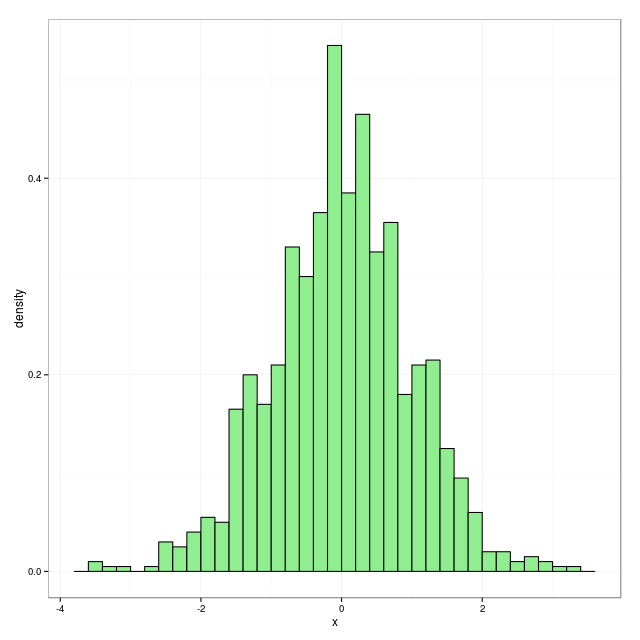
\includegraphics[width=0.5\linewidth]{pics/ris1}
	\caption{Связанная система координат квадрокоптера
	}
	\label{fig:ris1} % эта метка позволяет ссылаться на рисунок в тексте
\end{figure}
В качестве первого режима БПЛА \(U_{1}\) рассмотрим движение вдоль оси OZ, принадлежащей ССК. Данное движение обеспечивается одновременным увеличением скоростей винтов на одинаковое значение угловой скорости \(\Delta a\). Полученное при этом движение (рис. ~\ref{fig:ris1}) характеризуется взлетом или посадкой квадрокоптера (при нулевых значениях тангажа и крена) и описывается следующим выражением:
\begin{equation}
U_{1}=b(\Omega_{1}^2+\Omega_{2}^2+\Omega_{3}^2+\Omega_{4}^2)
\end{equation}
где b – аэродинамическая составляющая тяги винта.
В качестве второго режима движения БПЛА \(U_{2}\) необходимо взять поворот вокруг оси OX, принадлежащей ССК. Данное движение достигается путем увеличения/уменьшения на величину \(\Delta a\) значения \(\Omega_{4}\) левого винта и уменьшением/увеличением на величину \(\Delta b\) значения \(\Omega_{1}\)
правого. Полученное при этом движение характеризуется изменением угла крена \(\phi\) (рис. ~\ref{fig:ris2}) и описывается следующим выражением:
\begin{equation}
U_{2}=lb(-\Omega_{2}^2-\Omega_{4}^2)
\end{equation}
где l – расстояние между центром квадрокоптера и центром винта.
% ~\ref{fig:ris2}
\begin{figure}[H]
	\centering
	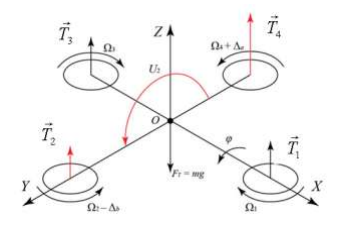
\includegraphics[width=0.5\linewidth]{pics/ris2}
	\caption{Вращение квадрокоптера вокруг оси OX
	}
	\label{fig:ris2} % эта метка позволяет ссылаться на рисунок в тексте
\end{figure}
В качестве третьего режима движения \(U_{3}\) необходимо взять поворот БПЛА вокруг оси OY , принадлежащей ССК. Данное движение достигается путем уменьшения/увеличения на величину \(\Delta a\) значения \(\Omega_{1}\) фронтального винта и увеличения/уменьшения на величину \(\Delta b\) значения \(\Omega_{3}\) заднего. Полученное при этом движение характеризуется изменением угла тангажа \(\theta\) (рис. ~\ref{fig:ris3}) и описывается следующим выражением:
\begin{equation}
U_{3}=lb(-\Omega_{1}^2-\Omega_{3}^2)
\end{equation}
% ~\ref{fig:ris3}
\begin{figure}[H]
	\centering
	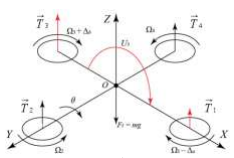
\includegraphics[width=0.5\linewidth]{pics/ris3}
	\caption{Вращение вокруг оси OY
	}
	\label{fig:ris3} % эта метка позволяет ссылаться на рисунок в тексте
\end{figure}
% ~\ref{fig:ris4}
\begin{figure}[H]
	\centering
	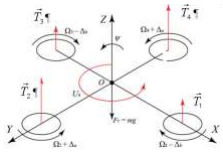
\includegraphics[width=0.5\linewidth]{pics/ris4}
	\caption{Вращение вокруг оси OZ
	}
	\label{fig:ris4} % эта метка позволяет ссылаться на рисунок в тексте
\end{figure}

 % переделать на две картинки рядом
В качестве последнего, четвертого, режима движения \(U_{4}\) необходимо взять поворот БПЛА вокруг оси OZ , принадлежащей ССК. Данное движение достигается путем одновременного увеличения/уменьшения на величину \(\Delta a\) значений \(\Omega_{4}\) левого и \(\Omega_{2}\) правого винтов, а также одновременного уменьшения/увеличения на величину \(\Delta b\) значений \(\Omega_{1}\) фронтального и \(\Omega_{3}\) заднего винтов. Благодаря вращению роторов в диагонально противоположных направлениях, полученное движение характеризуется изменением угла рыскания \(\psi\) (рис. ~\ref{fig:ris4}) и описывается следующим выражением:
\begin{equation}
U_{4}=d(-\Omega_{1}^2+\Omega_{2}^2-\Omega_{3}^2+\Omega_{4}^2)
\end{equation}
где d – аэродинамическая составляющая коэффициента сопротивления среды.
Введенное, с учетом (1) – (4), множество U, характеризующее режимы
движения квадрокоптера можно записать следующим образом:
\begin{numcases}{U=}
U_{1}=b(\Omega_{1}^2+\Omega_{2}^2+\Omega_{3}^2+\Omega_{4}^2)\\
U_{2}=lb(-\Omega_{2}^2-\Omega_{4}^2)\\
U_{3}=lb(-\Omega_{1}^2-\Omega_{3}^2)\\
U_{4}=d(-\Omega_{1}^2+\Omega_{2}^2-\Omega_{3}^2+\Omega_{4}^2)
\end{numcases}
Множество U определяет связь между системой исполнительных приводов и платформой БПЛА. Поэтому, при дальнейшем рассмотрении математической модели динамики движения квадрокоптера, режимы движения (1) – (4) будут использоваться как задающие воздействия для платформы БПЛА. \cite{mathmodel}

\subsection{Физическая модель квадрокоптера}

Квадрокоптер -- беспилотный летательный аппарат мультироторного типа с четырмя несущими винтами.
Квадрокоптер состоит из:

--- рамы,

--- 4 моторов,

--- 4 регуляторов оборотов,

--- полетного контроллера,

--- камеры,

--- видеопередатчика,

--- видеоантенны,

--- радиоприемника,

--- другой периферии (например, gps, магнитометра, дальномера, телеметрийного модуля)

 % ~\ref{fig:pix}
 \begin{figure}[H]
 	\centering
 	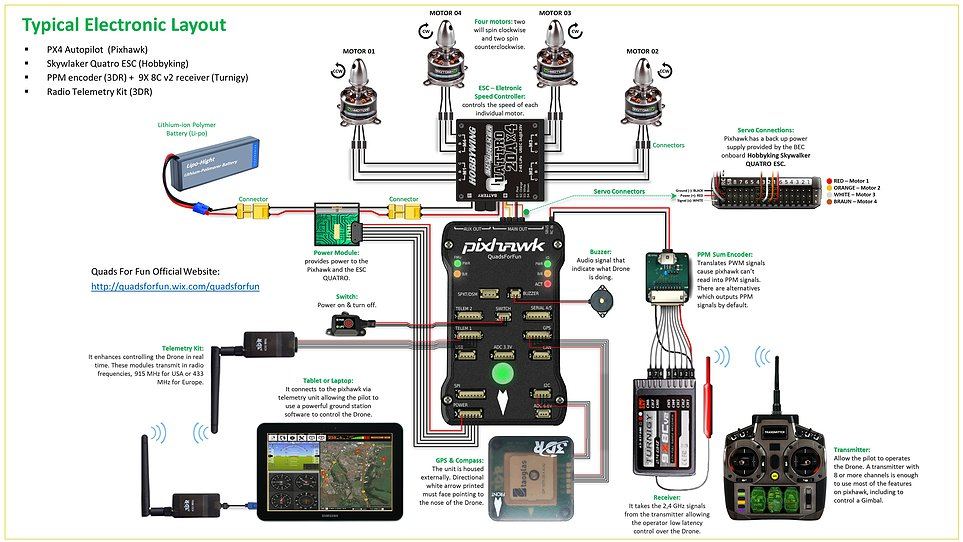
\includegraphics[width=0.9\linewidth]{pics/pix}
 	\caption{Пример схемы подключения
 	}
 	\label{fig:pix}
 \end{figure}
Рама - несущий компонент, на котором располагается вся электроника квадрокоптера. В большинстве случаев представляет собой крестообразную конструкцию. Рама должна быть жесткой, чтобы не создавать осцилляции для ПИД регулятора, и в то же время легкой. На данный момент лучшим материалом для рам квадрокоптеров является карбон.

Для современных БПЛА используются бесколлекторные моторы. Основными их характеристиками являются размер и количество оборотов на вольт. В зависимости от перечисленных характеристик, веса летательного аппарата, выбранного аккумулятора, поставленных задач подбираются пропеллеры.
Диаметр пропеллера и количество лопастей определяют статическую тягу квадрокоптера. Шаг пропеллера определяет скорость потока воздуха.

Регулятор оборотов передает энергию от батареи к двигателю, преобразуя постоянный ток источника питания в переменный ток, который нужен мотору. Количество оборотов мотора определяет полетный контроллер.

Для питания квадрокоптера используются литий-полимерные и литий-ионные аккумуляторы. В зависимости от задач и размеров подбирается количество ячеек аккумулятора, емкость и токоотдача.

Полетный контроллер -- система реального времени, которая интерпретирует входящие данные от приемника и бортовых датчиков (гироскопа, акселерометра, барометра), на основе которых рассчитывает и передает ШИМ на регуляторы оборотов, и тем самым производится регулировка скорости моторов. Все алгоритмы работы полетного контроллера содержатся в прошивке -- программном обеспечении, которое выбирается в зависимости от схемы полетного контроллера и поставленных задач.

Видеосистема состоит из трех основных компонентов: камера, видеопередатчик и передающая антенна. Видеопередатчик, в большинстве случаев, на частоте 5.8ГГц и указанной мощности передает изображение с камеры.

Для осуществления управления квадрокоптером используются радиопередатчики. Для приема сигнала к полетному контроллеру подключается приемник, общающийся с передатчиком по определенному протоколу на указанном диапазоне частот. В случае, если необходима обработка видеопотока или сбор информации, на квадрокоптер также ставится бортовой компьютер, так как обладает большими вычислительными мощностями. Как правило, бортовой компьютер представляет собой микрокомпьютер по типу raspberry pi или nvidia jetson. Информация с датчиков квадрокоптера оператору может передаваться с помощью телеметрийных модулей.

Теперь разберем, какие есть прошивки для полетных контроллеров.

\subsection{Семейства прошивок полетного контроллера}
Закрытые платные прошивки не интересуют, так как их невозможно модифицировать под наши нужды. Если взять во внимание наиболее популярные открытые прошивки для полетных контроллеров, то можно выделить 2 семейства: потомки MultiWii и прошивки под полетные контроллеры семейства PixHawk.

MultiWii - прошивка, изначально разработанная для получения и обработки данных с гироскопов и акселерометров игровой консоли Nintendo Wii. Позже был спроектирован полетный контроллер, куда был прошит MultiWii. Со временем MultiWii перерос в BaseFlight, а он в свою очередь в CleanFlight. Разработчики CleanFlight разошлись во мнениях касаемо функционала прошивки и сделали следующие ответвления:

---BetaFlight,

---INav,

---EmuFlight

BetaFlight нацелен на гоночные квадрокоптеры. Основными особенностями являются: минимальная фазовая задержка, точное следование управляющему сигналу и поддержка огромного количества полетных контроллеров.

INav сфокусирован на навигационных возможностях. Позволяет выполнять полеты по точкам, исходя из данных, полученных периферией. Поддерживает различные платформы, включая БПЛА мультироторного и самолетного типов, сухопутные и водные управляемые модели.

EmuFlight предназначен для полетов в свободном стиле. Позволяет настроить квадрокоптер на плавный полет, содержит множество алгоритмов для фильтрации шумов.

Для семейства PixHawk наиболее популярны PX4 и Ardupilot. Эти прошивки активно используются как хоббистами, так и специалистами в промышленной сфере. Они имеют множество проверенных временем функций, позволяющих выполнять автономные миссии. Ardupilot, в основном, разрабатывается и используется хоббийным сообществом. В то время как основным разработчиком PX4 является группа AeroAstro из MIT.

%\url{https://www.technologyreview.com/innovator/lorenz-meier/}
Изначально это был научный проект, но сейчас его используют исследователи в области программирования, стабилизации и навигации БПЛА во всем мире. Главными особенностями PX4 являются поддержка огромного количества датчиков и навигация в режиме OFFBOARD, который позволяет управлять беспилотником при помощи бортового компьютера. Именно этот режим нам и нужен, чтобы наземная станция управляла квадрокоптером. Рассмотрим PX4 подробнее.

\subsection{PX4}
\url{https://docs.px4.io/master/en/getting_started/px4_basic_concepts.html}

\url{https://docs.px4.io/master/en/contribute/licenses.html}

PX4 - прошивка с открытым исходным кодом, публикуемая под лицензией BSD. PX4 позволяет управлять различными типами беспилотников, включая: летательные (мультикоптеры, самолеты и вертолеты), наземные и подводные аппараты. Он совместим с большим количеством оборудования, датчиков и другой периферии. Позволяет реализовать гибкие режимы полета и функции безопасности.
Параметры PX4 настраиваются с помощью QGroundControl.\cite{px4}

QGroundControl - кросплатформенный конфигуратор для настройки PX4 и Ardupilot прошивок. Он обеспечивает полное управление полетом и настройку беспилотника. \cite{qgroundcontrol}

PX4 для определения состояния аппарата, его стабилизации и автономного полета использует датчики, такие как: гироскоп, акселерометр, магнитометр (компас) и барометр. Для включения всех автоматических режимов и некоторых вспомогательных требуется GPS или другая система позиционирования.
Для передачи данных / телеметрии между наземной станцией управления, такой как QGroundControl, и беспилотником, работающим под управлением PX4 может использоваться как проводное, так и беспроводное соединение по протоколу MAVLink. Он позволяет настраивать параметры во время полета, проверять телеметрию в режиме реального времени, менять миссию на лету и т. д.

%Автономный / вспомогательный компьютер
PX4 можно управлять с отдельного компьютера-компаньона через последовательный кабель или Wi-Fi. Компаньон-компаньон обычно обмениваются данными с помощью API MAVLink, такого как MAVSDK или MAVROS.
\cite{px4}

\subsection{MAVLink}
%зачем писать, если есть 
\url{https://mavlink.io/en/}

MAVLink -- это очень легкий протокол обмена сообщениями для связи с дронами (и между бортовыми компонентами дронов).

MAVLink следует современному гибридному шаблону проектирования «публикация-подписка» и «точка-точка»: потоки данных отправляются / публикуются как темы, а подпротоколы конфигурации, такие как протокол задания или протокол параметров, являются point-to-point с повторной передачей.

Сообщения определяются в файлах XML. Каждый файл XML определяет набор сообщений, поддерживаемый MAVLink системой, также называемый «диалектом». Набор эталонных сообщений, который реализуется большинством наземных станций управления и автопилотов, определен в common.xml (большинство диалектов основано на этом определении).

Набор инструментов MAVLink использует определения XML сообщений для генерации библиотеки MAVLink для каждого из поддерживаемых языков программирования . Дроны, наземные станции управления и другие системы MAVLink используют сгенерированные библиотеки для связи. Они распространяются под лицензией MIT и поэтому могут использоваться без ограничений в любом приложении с закрытым исходным кодом без публикации исходного кода. MAVLink был впервые выпущен в начале 2009 года Лоренцем Мейером (основателем PX4) и в настоящее время имеет значительное количество разработчиков.

MAVLink поддерживает множество языков программирования, работающих на множестве микроконтроллеров / операционных систем (включая ARM7, ATMega, dsPic, STM32 и Windows, Linux, MacOS, Android и iOS). Допускает одновременно до 255 систем в сети (беспилотники, наземные станции и т. д.)

Обеспечивает как внешнюю, так и бортовую связь (например, между groundcontrol и дроном, а также между автопилотом дрона и камерой дрона с поддержкой MAVLink).
\cite{mavlink}

MAVLink развернут в двух основных версиях: v1.0 и v2.0, которые имеют обратную совместимость (реализации v2.0 могут анализировать и отправлять пакеты v1.0). Потоки телеметрических данных отправляются в многоадресном режиме, в то время как аспекты протокола, которые изменяют конфигурацию системы и требуют гарантированной доставки, являются point-to-point с повторной передачей.

//переделать

Для того, чтобы наземная станция могла общаться по MAVLink с БПЛА, необходима операционная система. Разработка ОС -- задача трудоемкая и не всегда обоснованная, так как существует множество готовых решений. ОС на базе ядра Linux имеют набор инструментов, позволяющий  Одним из них является ROS.
% дописать про офборд
\subsection{ROS}
\url{https://www.ros.org/about-ros/}

Robotic Operation System (ROS) - это гибкая платформа для написания программного обеспечения для роботов; набор инструментов, библиотек и соглашений, которые призваны упростить задачу создания сложного и надежного поведения роботов на самых разных роботизированных платформах.
\cite{ros}
Целью создания ROS является создание среды разработки, которая позволяет разработчикам ПО для роботов взаимодействовать на глобальном уровне.

ROS сосредоточена на максимизации повторного использования кода при разработке. Основные характеристики, позволяющие это реализовать:

Распределенный процессы. Структура ROS создана в виде минимальных единиц исполняемых процессов (нод), и каждый процесс выполняется изолированно. Взаимодействие разных нод происходит только на уровне обмена сообщениями.

Управление пакетами. Несколько процессов, имеющих общую задачу, объединяются в пакеты. Управление пакетами подразумевает набор утилит, позволяющих автоматически скачивать, устанавливать и удалять пакеты. Пакетный менеджер гарантирует работоспособность и целостность установленных пакетов.

Публичные репозитории и документация. Каждый доступный пакет публикуется в публичном репозитории. Документация пакетов публикуется в единой системе, которая упрощает поиск необходимых пакетов.

Единое API. При разработке программы, использующей ROS, вы получаете простое и легко встраиваемое API. При этом при использовании API нет разницы, на каком языке была написана программа.

Поддержка различных языков программирования. ROS предоставляет клиентские библиотеки для поддержки различных языков программирования. Наиболее популярны Python, C ++, а также такие языки, как Lisp, JAVA, C\#, Lua и Ruby.
\cite{voltbro}

Концепции

Ноды

Основная статья: \url{http://wiki.ros.org/Nodes}

ROS-нода – это специальная программа (обычно написанная на Python или C++), которая взаимодействует с другими нодами посредством ROS-топиков и ROS-сервисов. Разделение сложных робототехнических систем на изолированные ноды дает определенные преимущества: понижается связанность кода, повышается переиспользуемость и надежность.

Очень многие робототехнические библиотеки и драйвера выполнены именно в виде ROS-нод.

Для того, чтобы превратить обычную программу в ROS-ноду, необходимо подключить к ней библиотеку rospy или roscpp и добавить инициализирующий код.

Пример ROS-ноды на языке Python:


\begin{Program}[H]
	\caption{Пример ROS-ноды на языке Python:} \label{lst:1}
	\begin{MyCode}
import rospy

rospy.init\_node('my\_ros\_node')  # имя ROS-ноды

rospy.spin()  # входим в бесконечный цикл...
	\end{MyCode}
\end{Program}
Топики
Основная статья: http://wiki.ros.org/Topics

Топик – это именованная шина данных, по которой ноды обмениваются сообщениями. Любая нода может опубликовать сообщение в произвольный топик, а также подписаться на произвольный топик.

\begin{Program}[H]
	\caption{Пример публикации сообщения типа std\_msgs/String (строка) в топик /foo на языке Python:} \label{lst:1}
	\begin{MyCode}
from std\_msgs.msg import String

# ...

foo\_pub = rospy.Publisher('/foo', String, queue\_size=1)  # создаем Publisher'а

# ...

foo\_pub.publish(data='Hello, world!')  # публикуем сообщение
Пример подписки на топик /foo:

def foo\_callback(msg):
print msg.data

# Подписываемся. При получении сообщения в топик /foo будет вызвана функция foo\_callback.
rospy.Subscriber('/foo', String, foo\_callback)
	\end{MyCode}
\end{Program}

Также, существует возможность работы с топиками с помощью утилиты rostopic. Например, с помощью следующей команды можно просматривать сообщения, публикуемые в топик /mavros/state:

rostopic echo /mavros/state

Сервисы

Основная статья: \url{http://wiki.ros.org/Services}

Сервис – это некоторый аналог функции, которая может быть вызвана из одной ноды, а обработана в другой. У сервиса есть имя, аналогичное имени топика, и 2 типа сообщений: тип запроса и тип ответа.

\begin{Program}[H]
	\caption{Пример вызова ROS-сервиса из языка Python:} \label{lst:1}
	\begin{MyCode}
from clover.srv import GetTelemetry

# ...

# Создаем обертку над сервисом get\_telemetry пакета clover с типом GetTelemetry:
get\_telemetry = rospy.ServiceProxy('get\_telemetry', srv.GetTelemetry)

# Вызываем сервис и получаем телеметрию квадрокоптера:
telemetry = get\_telemetry()
С сервисами можно также работать при помощи утилиты rosservice. Так можно вызвать сервис /get\_telemetry из командной строки:

rosservice call /get\_telemetry "{frame\_id: ''}"
	\end{MyCode}
\end{Program}


\subsection{MAVROS}
\url{https://clover.coex.tech/ru/mavros.html}
\url{https://dev.px4.io/master/en/ros/mavros\_installation.html}

MAVROS (MAVLink + ROS) — это пакет для ROS, предоставляющий возможность управлять беспилотниками по протоколу MAVLink. MAVROS поддерживает полетные стеки PX4 и APM. Связь организовывается по UART, USB, TCP или UDP.

MAVROS подписывается на определенные ROS-топики в ожидании команд, публикует в другие топики телеметрию, и предоставляет сервисы.
Пакет mavros ROS обеспечивает расширяемую связь MAVLink между компьютерами, на которых работает ROS, автопилоты с поддержкой MAVLink и GCS с поддержкой MAVLink.

MAVROS - это «официальный» поддерживаемый мост между ROS и протоколом MAVLink. В настоящее время он расширяется, чтобы включить обмен сообщениями fast-RTPS , включая уровень для преобразования сообщений uORB PX4 в общие идиомы ROS.

Хотя MAVROS может использоваться для связи с любым автопилотом с поддержкой MAVLink, эта документация будет в контексте обеспечения связи между полетным стеком PX4 и компаньоном с поддержкой ROS.
